\section{Protection by in-block cancellation}
\label{sec:block}

Within a block, Hyperliquid processes cancellations before aggressors
(Section~\ref{sec:reconstruction}). A market maker who sees an informed aggressor coming
and cancels in the same block is therefore protected: the cancellation wins,
even though the aggressor's order and the cancellation are, in time, the same.
On a venue with continuous matching the same race would be decided by latency.

\subsection{Encounters}
We call an \emph{encounter} the first trade at an order's price after the order
reached the front of its queue, within its life. Under strict time priority such
a trade fills the order---unless the order was cancelled in the same block. An
encounter therefore ends in one of three ways: a fill, a rescue by in-block
cancellation, or otherwise. We also report encounters where the order had
reached the front in an earlier block, the only ones for which it is certain
that it led the level when the trade arrived.

\begin{table}[t]
\centering\small
\caption{How encounters end, pilot hour. ``Settled'': the order reached the front
in an earlier block than the trade.}
\label{tab:encounters}
\begin{tabular}{@{}lrr@{}}
\toprule
 & \SOL & \BTC \\
\midrule
Encounters & 4\,618 & 26\,528 \\
Filled & 94.95\% & 97.18\% \\
\textbf{Rescued by in-block cancellation} & \textbf{4.35\%} & \textbf{2.36\%} \\
Rescued, settled encounters & 5.54\% & 3.11\% \\
\bottomrule
\end{tabular}
\end{table}

Roughly one encounter in twenty to thirty ends not in a fill but in a
cancellation that the exchange processed before the trade
(Table~\ref{tab:encounters}). Over the full sample the rescued share is
\tbd{} for \BTC, \tbd{} for \ETH{} and \tbd{} for \SOL, and it ranges from \tbd{}
to \tbd{} across hours.

\subsection{The block rule in fill models}
We add to each rule a block variant: a trade in the block in which a not-yet-filled
order was cancelled does not fill it. Table~\ref{tab:blockrule} shows the effect.
With the block rule, \qa{} matches the observed fill rate exactly, leaving 16 and
42 false fills among half a million and one and a half million unfilled orders.
The block rule also removes 12--13\% of \touch's false fills, so cancellations
often fall in blocks with trading at the order's price even when the order is
not yet at the front.

\begin{table}[t]
\centering\small
\caption{Fill rules without and with the exchange's in-block order
(``block'': a trade in the block where the order was cancelled does not fill
it): fill rate over the observed one, and false fills.}
\label{tab:blockrule}
\setlength{\tabcolsep}{4pt}
\begin{tabular}{@{}l cc rr@{}}
\toprule
 & \multicolumn{2}{c}{$\times$ real} & \multicolumn{2}{c}{false fills} \\
\cmidrule{2-3}\cmidrule{4-5}
Rule & plain & block & plain & block \\
\midrule
\multicolumn{5}{@{}l}{\SOL} \\
\touch & 6.07 & 5.40 & 22\,323 & 19\,385 \\
\vt    & 0.34 & 0.32 & 99 & 3 \\
\qa    & 1.05 & \textbf{1.00} & 217 & \textbf{16} \\
\multicolumn{5}{@{}l}{\BTC} \\
\touch & 4.71 & 4.27 & 96\,085 & 84\,669 \\
\vt    & 0.47 & 0.45 & 611 & 23 \\
\qa    & 1.02 & \textbf{1.00} & 667 & \textbf{42} \\
\bottomrule
\end{tabular}
\end{table}

Stated as the cost of ignoring block semantics: a fill model unaware of the
in-block processing order credits a strategy with 4.6\% too many fills on \SOL{}
(201 against 4\,405 real ones) and 2.4\% on \BTC{} (625 against 25\,894)---exactly
the fills from which a cancellation in fact protected the order.

\subsection{What the rescued fills would have been worth}
The markout of a fill at horizon $h$ is its gain against the mid-price $h$
later, in basis points of its price, signed by side: positive if the fill paid,
negative if the price went on through the order. For real fills it is taken at
the fill; for rescued ones at the encounter, as if the fill had happened. A
horizon past the end of observation is left undefined.

\begin{figure}[t]
\centering
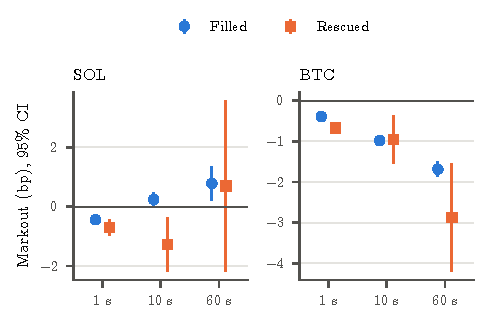
\includegraphics[width=\columnwidth]{markout}
\caption{Markout of real fills and of fills rescued by in-block cancellation,
mean with 95\% confidence interval, at three horizons. Pilot hour.}
\label{fig:markout}
\end{figure}

Rescued fills would have been worse than real ones at the one-second horizon, by
0.27--0.28\bps{} on both instruments (4.6 standard errors on \BTC), and on \SOL{}
also at ten seconds, by 1.52\bps{} (3.2 standard errors;
Figure~\ref{fig:markout}). This is consistent with the
rescuing cancellations being a response to the same information that moved the
aggressor: in-block priority protects market makers precisely against toxic
flow. At one minute the difference is not distinguishable in this sample.
Pooled over the full sample, with standard errors clustered by hour, the
one-second gap is \tbd\bps{} (\tbd{} s.e.) for \BTC, \tbd\bps{} (\tbd{} s.e.) for
\ETH{} and \tbd\bps{} (\tbd{} s.e.) for \SOL.
